\documentclass{article}
\usepackage[a4paper, margin=1in]{geometry}
\usepackage{graphicx}
\usepackage{subcaption}
\usepackage{float}

\graphicspath{ {../images/} }


\begin{document}

\begin{figure}
    \centering
    \begin{subfigure}{\textwidth}
        \centering
        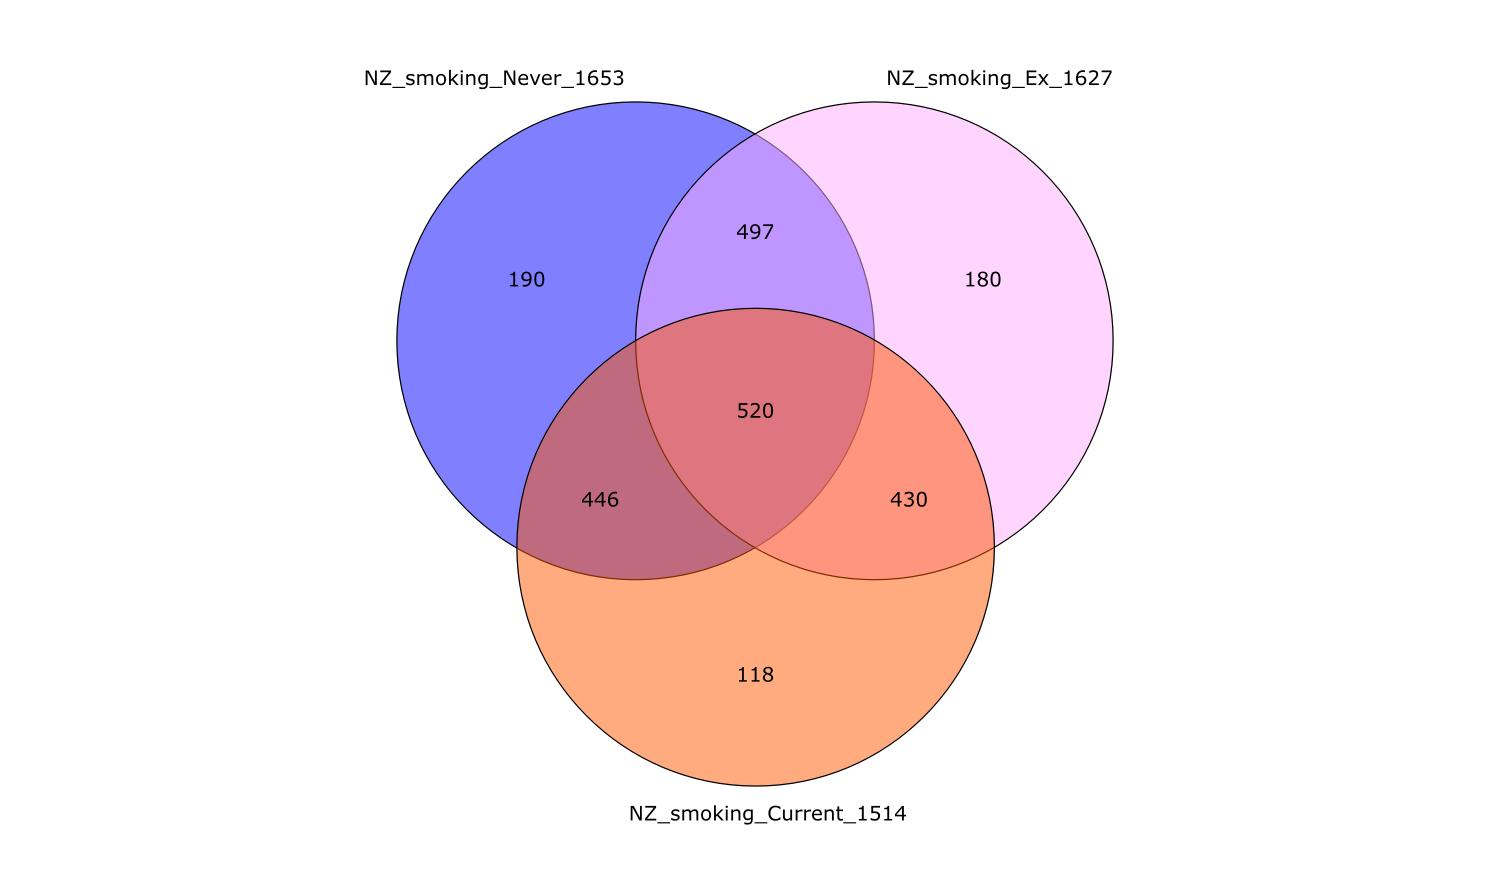
\includegraphics[width=\linewidth]{Venn_NZ_3gps.jpg}
        \caption{Intersection of sets of CpG sites used to predict never-, ex- and current-smokers. While a total of 2381 CpG sites are used in the entire model, only 520 CpG sites are used in all three predictions, and each sub-predictor only uses approximately 1600 CpG sites.}
    \end{subfigure}
    \begin{subfigure}{\textwidth}
        \centering
        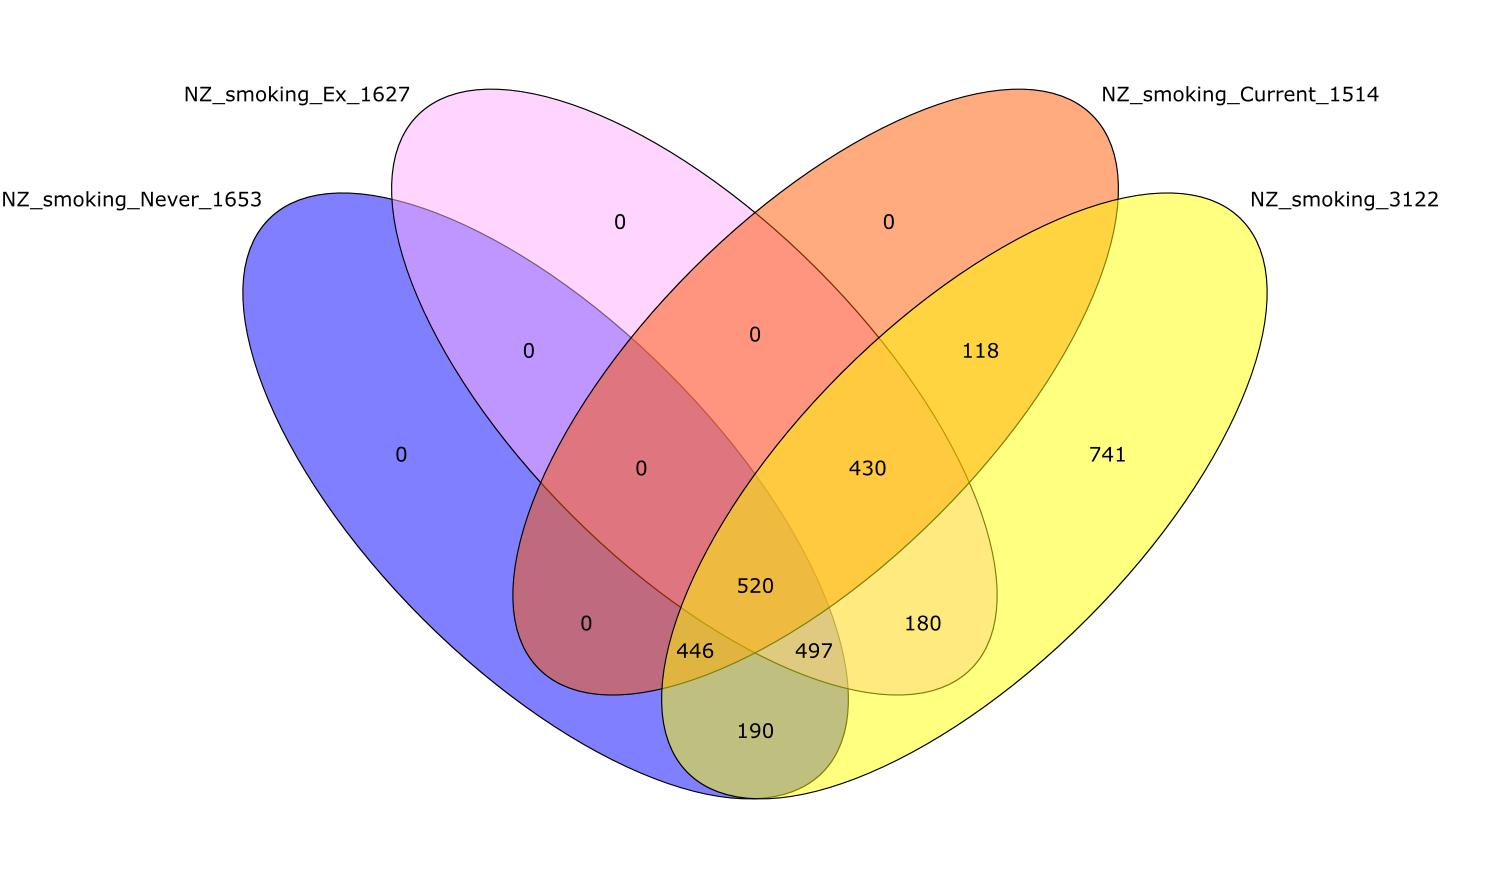
\includegraphics[width=\linewidth]{Venn_NZ_3gps_KWlist.jpg}
        \caption{Same diagram above intersected with the original 3122 CpG sites returned from Kruskal-Wallis.}
    \end{subfigure}
    \caption{Intersections of sets of CpG sites used in model}
    \label{fig:model-intersect}
\end{figure}

\begin{figure}
    \centering
    \begin{subfigure}{0.75\textwidth}
        \centering
        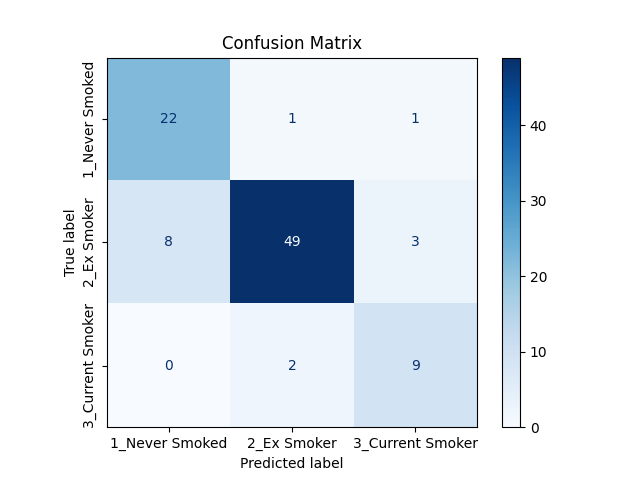
\includegraphics[width=\linewidth]{cohort1_cm.png}
        \caption{Confusion Matrix for Cohort 1 test set. The model makes very few incorrect predictions.}
    \end{subfigure}
    % \hfill
    \begin{subfigure}{0.75\textwidth}
        \centering
        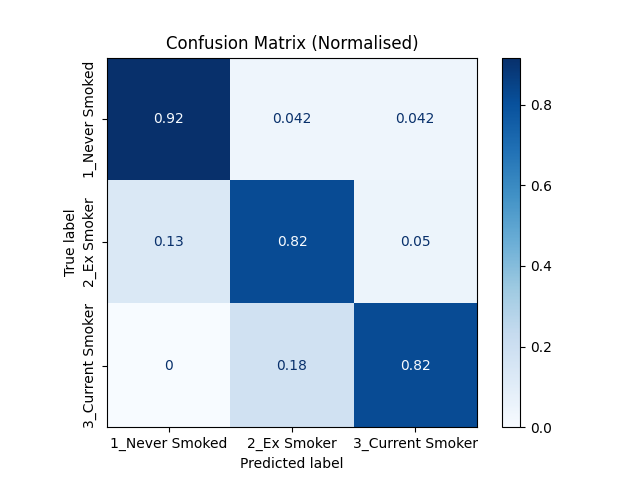
\includegraphics[width=\linewidth]{cohort1_cm_n.png}
        \caption{Confusion Matrix (normalised) for Cohort 1 test set. As before, we can see the model achieves near-perfect predictive performance.}
    \end{subfigure}
    \caption{Confusion Matrices (Cohort 1 test set)}
    \label{fig:cohort1-cm}
\end{figure}

\begin{figure}
    \begin{subfigure}{0.43\textwidth}
        \centering
        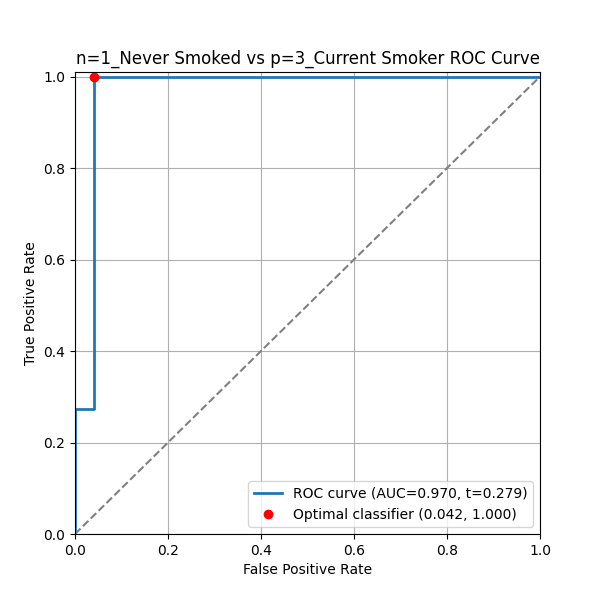
\includegraphics[width=\linewidth]{cohort1_1v3_roc.png}
        \caption{Separation of never- vs current-smokers by current-smoker sub-predictor}
    \end{subfigure}
    \hfill
    \begin{subfigure}{0.43\textwidth}
        \centering
        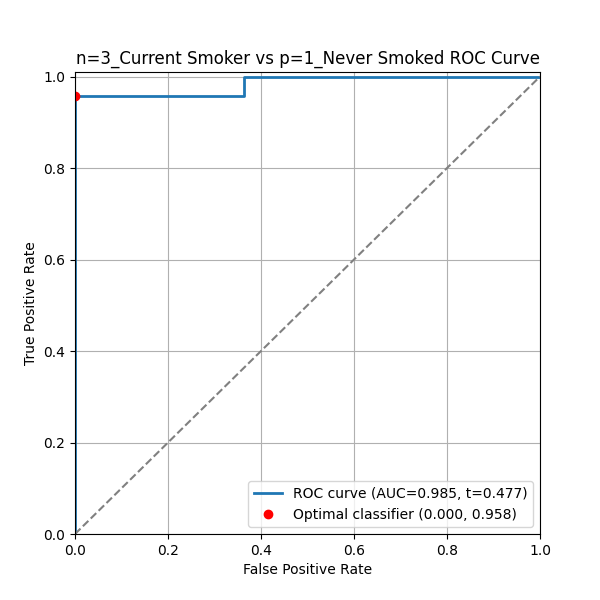
\includegraphics[width=\linewidth]{cohort1_3v1_roc.png}
        \caption{Separation of never- vs current-smokers by never-smoker sub-predictor}
    \end{subfigure}
    % \caption{Never- smoker vs current- smoker sub-predictors performance (Cohort 1)}

    \begin{subfigure}{0.43\textwidth}
        \centering
        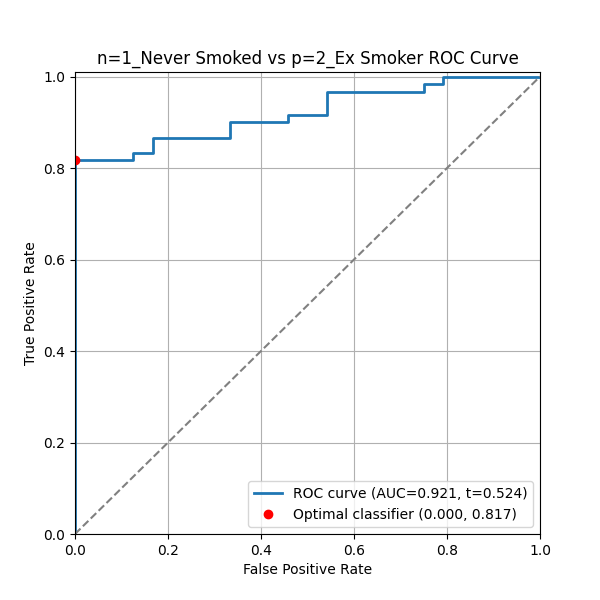
\includegraphics[width=\linewidth]{cohort1_1v2_roc.png}
        \caption{Separation of never- vs ex-smokers by ex-smoker sub-predictor}
    \end{subfigure}
    \hfill
    \begin{subfigure}{0.43\textwidth}
        \centering
        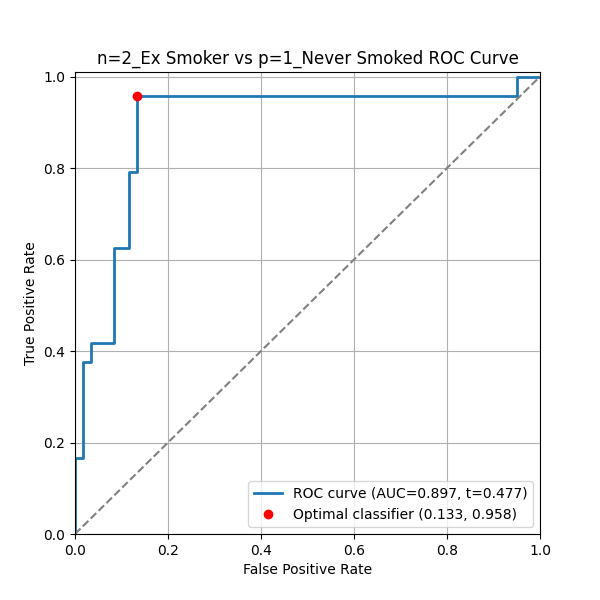
\includegraphics[width=\linewidth]{cohort1_2v1_roc.png}
        \caption{Separation of never- vs ex-smokers by never-smoker sub-predictor}
    \end{subfigure}
    % \caption{Never- smoker vs ex-smoker sub-predictors performance (Cohort 1)}

    \begin{subfigure}{0.43\textwidth}
        \centering
        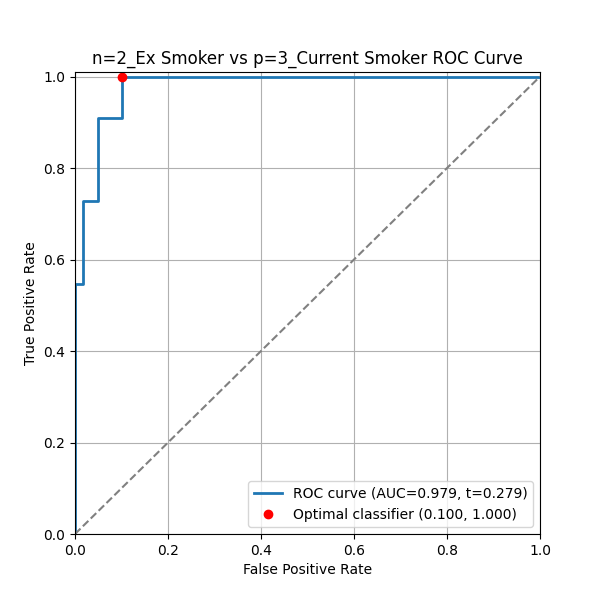
\includegraphics[width=\linewidth]{cohort1_2v3_roc.png}
        \caption{Separation of ex vs current-smokers by current-smoker sub-predictor}
    \end{subfigure}
    \hfill
    \begin{subfigure}{0.43\textwidth}
        \centering
        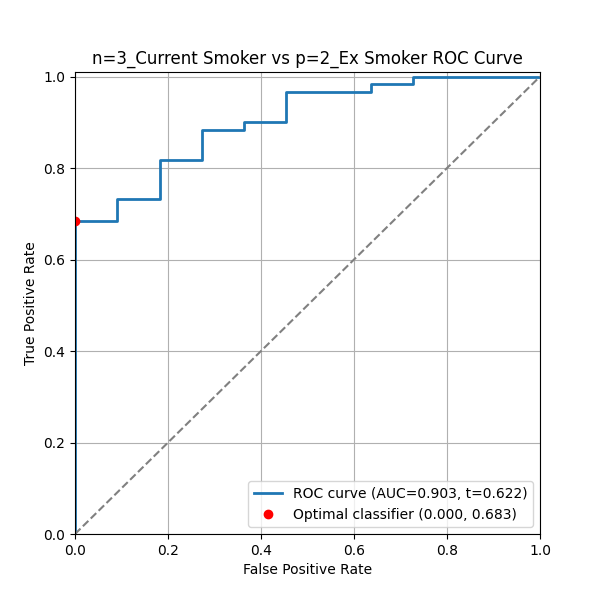
\includegraphics[width=\linewidth]{cohort1_3v2_roc.png}
        \caption{Separation of ex vs current-smokers by ex-smoker sub-predictor}
    \end{subfigure}
    % \caption{Ex-smoker vs current- smoker sub-predictors performance (Cohort 1)}
    \caption{One vs one sub-predictor performance (Cohort 1 test set)}
    \label{fig:ovo-roc-cohort1}
\end{figure}

\begin{figure}
    \centering
    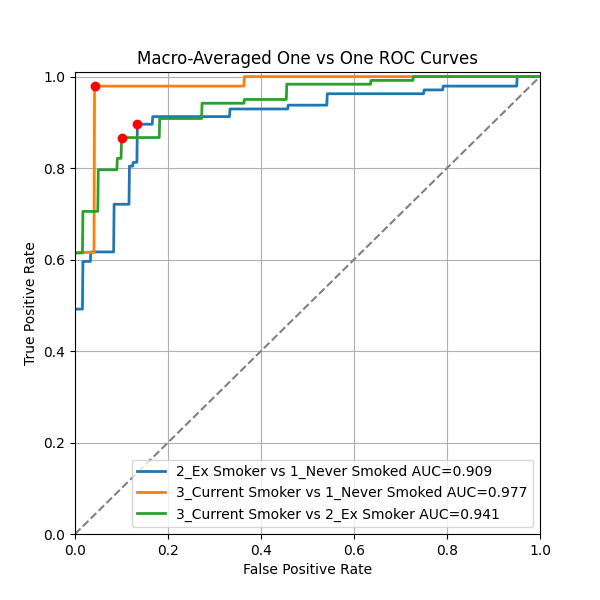
\includegraphics[width=0.75\linewidth]{cohort1_macro_ovo_roc.png}
    \caption{Class separation of classifier (Cohort 1 test set)}
    \label{fig:macro-roc-cohort1}
\end{figure}

\begin{figure}
    \centering
    \begin{subfigure}{0.48\textwidth}
        \centering
        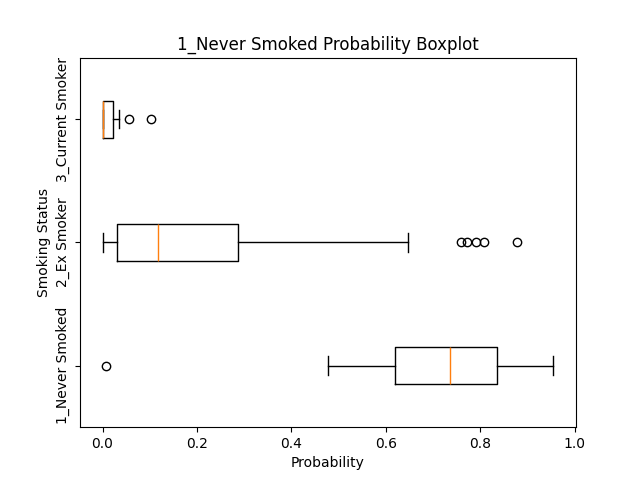
\includegraphics[width=\linewidth]{cohort1_1_boxplot.png}
        \caption{Never-smoker sub-predictor probabilities across all three classes}
    \end{subfigure}
    \hfill
    \begin{subfigure}{0.48\textwidth}
        \centering
        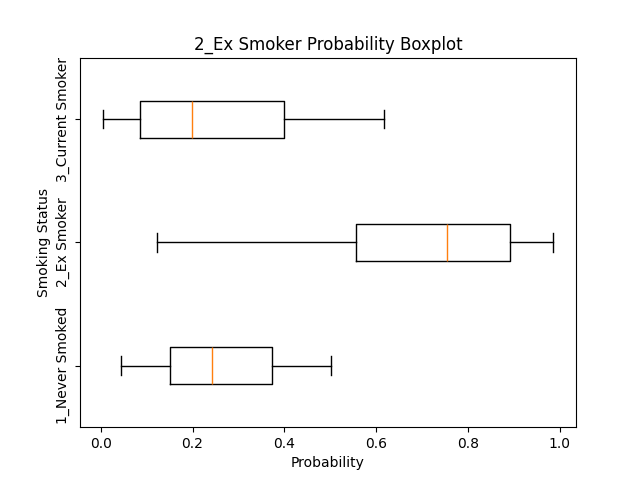
\includegraphics[width=\linewidth]{cohort1_2_boxplot.png}
        \caption{Ex-smoker sub-predictor probabilities across all three classes}
    \end{subfigure}
    \par\vspace{0.5em}
    \begin{subfigure}{0.48\textwidth}
        \centering
        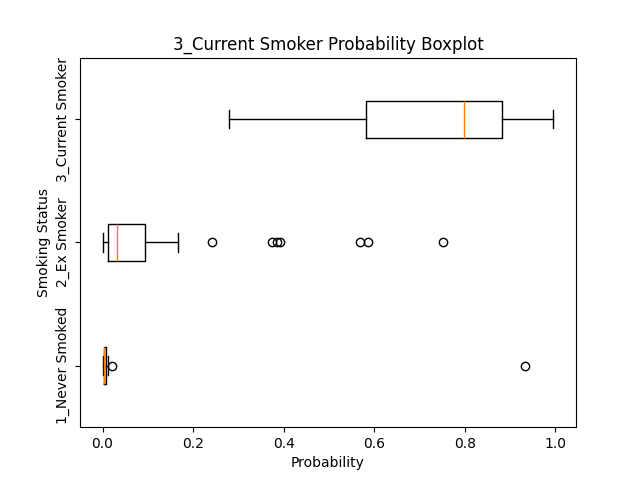
\includegraphics[width=\linewidth]{cohort1_3_boxplot.png}
        \caption{Current- smoker sub-predictor probabilities across all three classes}
    \end{subfigure}
    \caption{Boxplots of probability distributions (Cohort 1)}
    \label{fig:boxplot-cohort1}
\end{figure}


\begin{figure}
    \begin{subfigure}{0.49\textwidth}
        \centering
        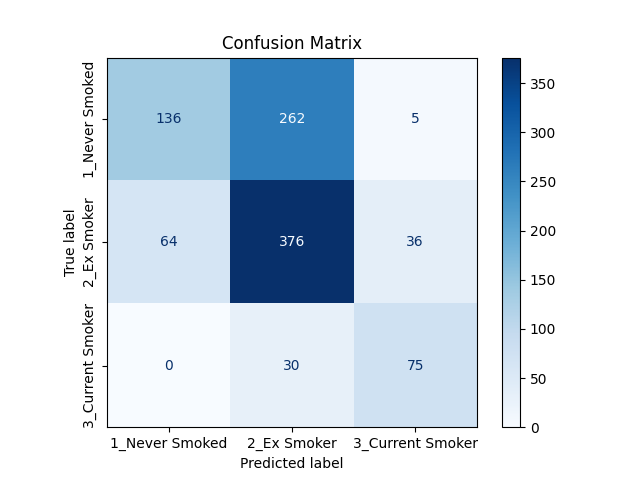
\includegraphics[width=\linewidth]{cohort2_cm.png}
        \caption{CM}
    \end{subfigure}
    \hfill
    \begin{subfigure}{0.49\textwidth}
        \centering
        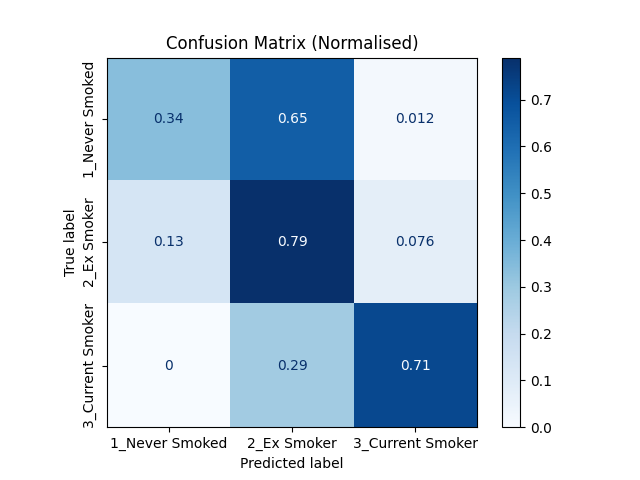
\includegraphics[width=\linewidth]{cohort2_cm_n.png}
        \caption{CM Normalised}
    \end{subfigure}
    \caption{Confusion Matrices (Cohort 2)}
\end{figure}

\begin{figure}
    \begin{subfigure}{0.48\textwidth}
        \centering
        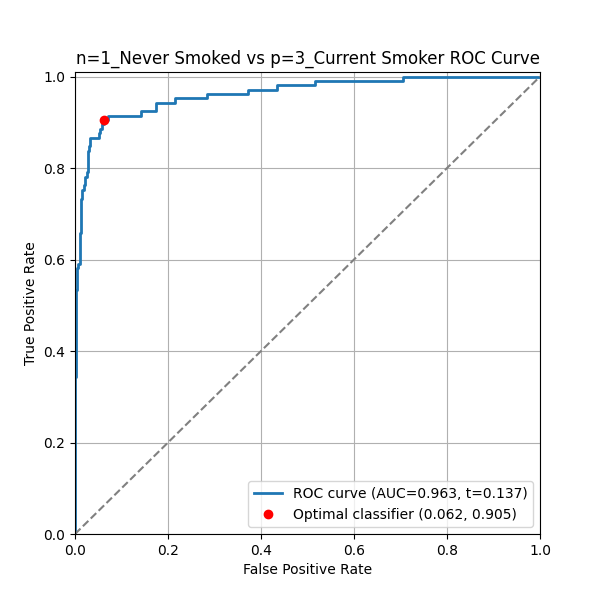
\includegraphics[width=\linewidth]{cohort2_1v3_roc.png}
        \caption{Seperation of never vs current smokers by current smoker sub-classifier}
    \end{subfigure}
    \hfill
    \begin{subfigure}{0.48\textwidth}
        \centering
        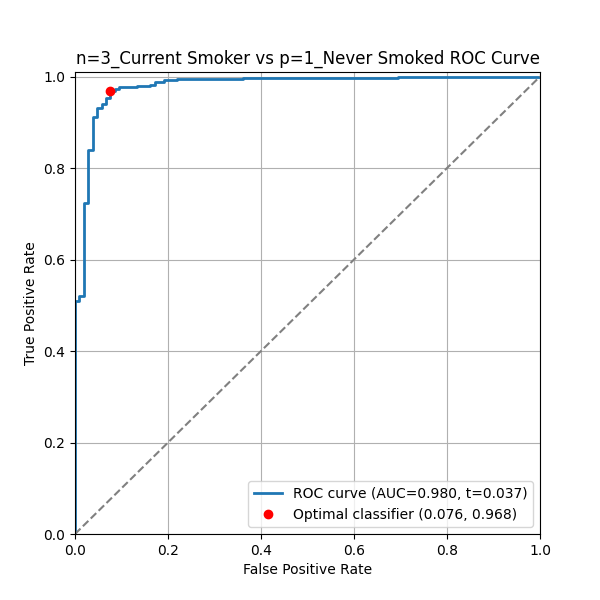
\includegraphics[width=\linewidth]{cohort2_3v1_roc.png}
        \caption{Seperation of never vs current smokers by never smoker sub-classifier}
    \end{subfigure}
    \caption{Never smoker vs current smoker sub-classifiers performance (Cohort 2)}
\end{figure}

\begin{figure}
    \begin{subfigure}{0.48\textwidth}
        \centering
        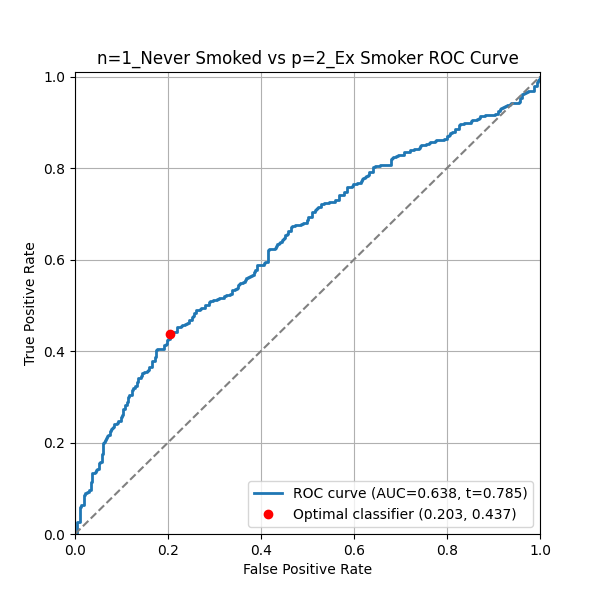
\includegraphics[width=\linewidth]{cohort2_1v2_roc.png}
        \caption{Seperation of never vs ex-smokers by ex-smoker sub-classifier}
    \end{subfigure}
    \hfill
    \begin{subfigure}{0.48\textwidth}
        \centering
        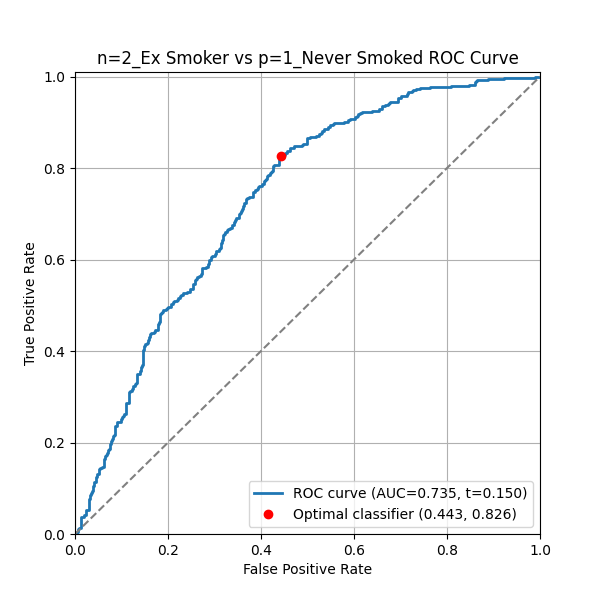
\includegraphics[width=\linewidth]{cohort2_2v1_roc.png}
        \caption{Seperation of never vs ex-smokers by never smoker sub-classifier}
    \end{subfigure}
    \caption{Never smoker vs ex-smoker sub-classifiers performance (Cohort 2)}
\end{figure}

\begin{figure}
    \begin{subfigure}{0.48\textwidth}
        \centering
        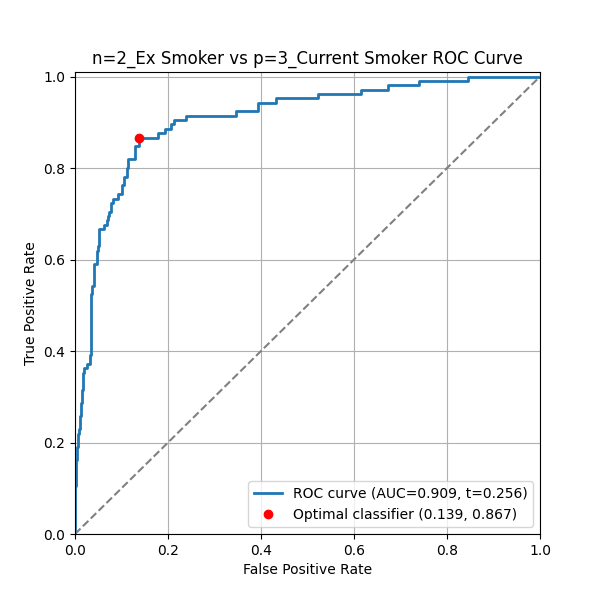
\includegraphics[width=\linewidth]{cohort2_2v3_roc.png}
        \caption{Seperation of ex vs current smokers by current smoker sub-classifier}
    \end{subfigure}
    \hfill
    \begin{subfigure}{0.48\textwidth}
        \centering
        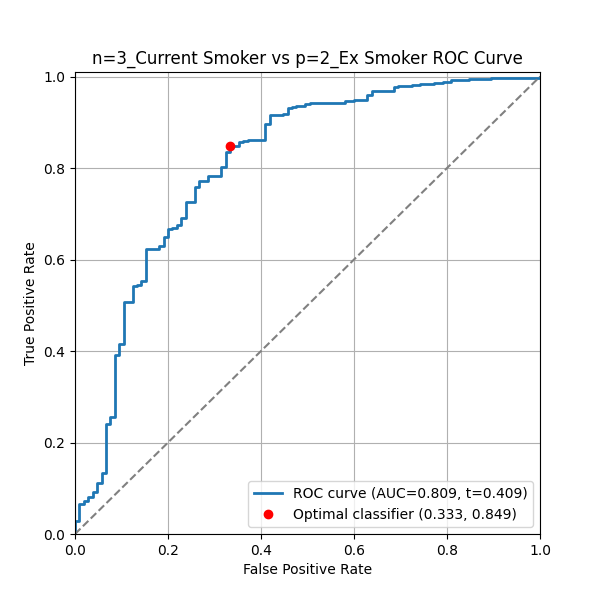
\includegraphics[width=\linewidth]{cohort2_3v2_roc.png}
        \caption{Seperation of ex vs current smokers by ex-smoker sub-classifier}
    \end{subfigure}
    \caption{Ex-smoker vs current smoker sub-classifiers performance (Cohort 2)}
\end{figure}

\begin{figure}
    \centering
    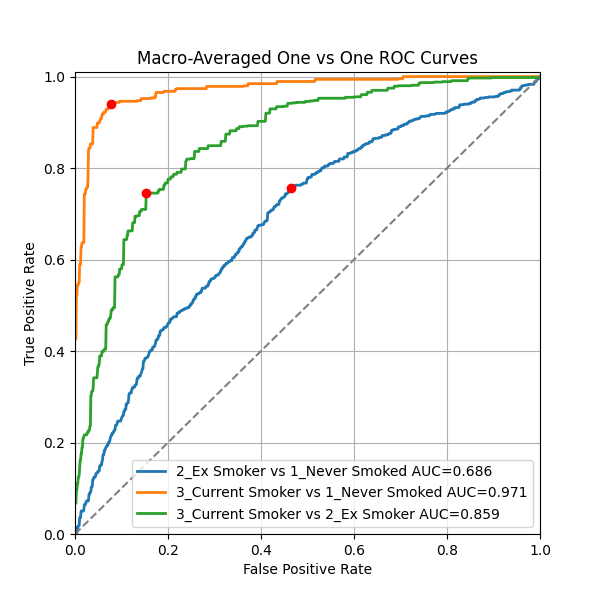
\includegraphics[width=\linewidth]{cohort2_macro_ovo_roc.png}
    \caption{Class seperation of classifier (Cohort 2)}
\end{figure}

\begin{figure}
    \centering
    \begin{subfigure}{0.48\textwidth}
        \centering
        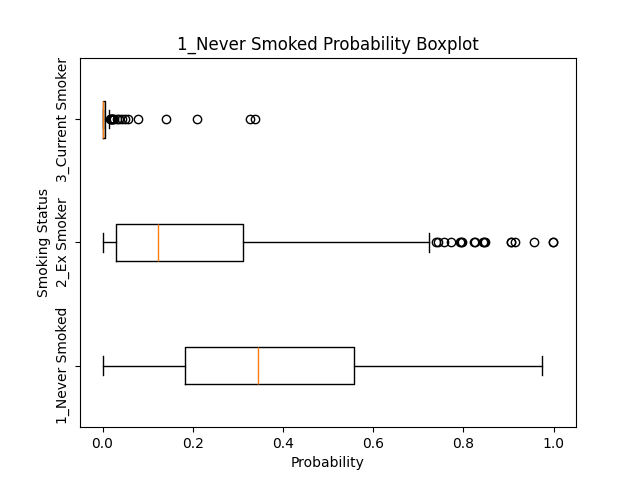
\includegraphics[width=\linewidth]{cohort2_1_boxplot.png}
        \caption{Never smoker sub-classifier probabilities across all three classes}
    \end{subfigure}
    \hfill
    \begin{subfigure}{0.48\textwidth}
        \centering
        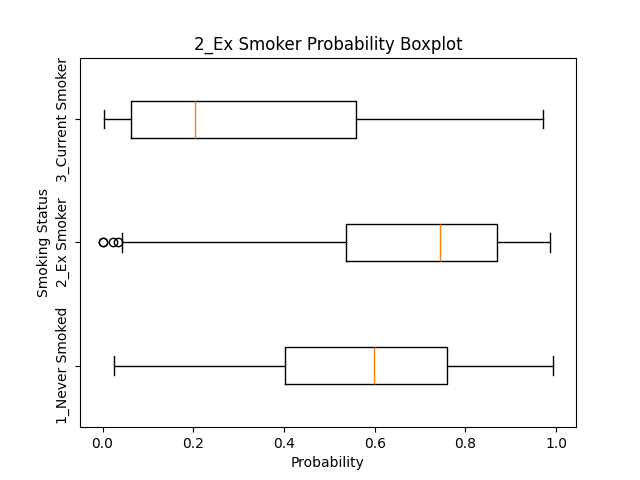
\includegraphics[width=\linewidth]{cohort2_2_boxplot.png}
        \caption{Ex-smoker sub-classifier probabilities across all three classes}
    \end{subfigure}
    \par\vspace{0.5em}
    \begin{subfigure}{0.48\textwidth}
        \centering
        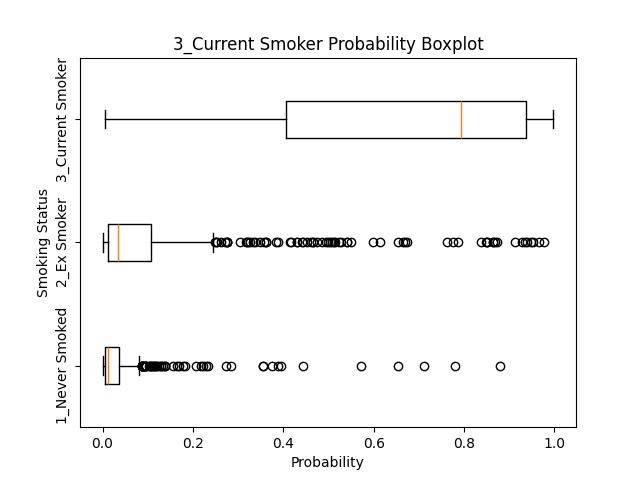
\includegraphics[width=\linewidth]{cohort2_3_boxplot.png}
        \caption{Current smoker sub-classifier probabilities across all three classes}
    \end{subfigure}
    \caption{Boxplots of probability distributions (Cohort 2)}
\end{figure}

\begin{figure}
    \centering
    \begin{subfigure}{0.48\textwidth}
        \centering
        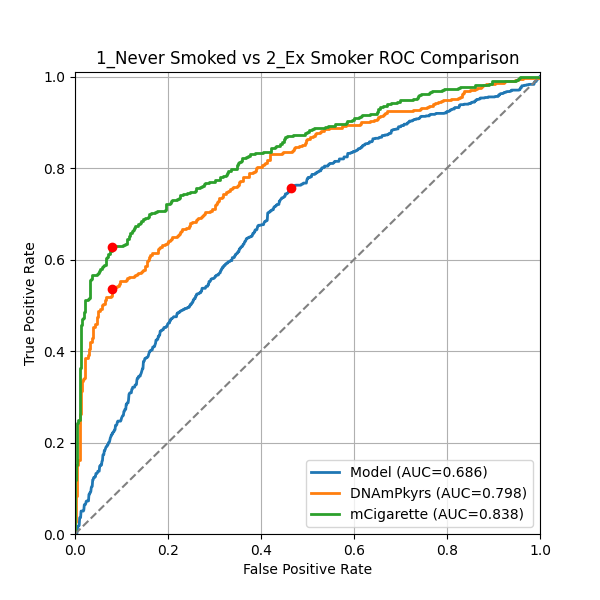
\includegraphics[width=\linewidth]{comparison_1v2_roc.png}
        \caption{comparison 1v2}
    \end{subfigure}
    \hfill
    \begin{subfigure}{0.48\textwidth}
        \centering
        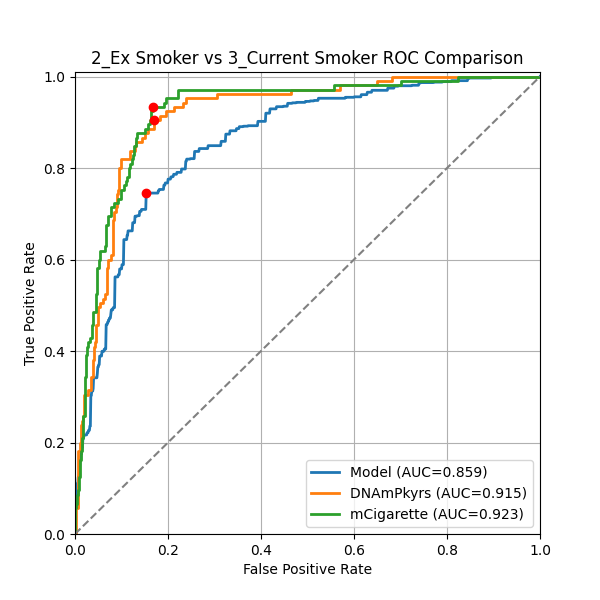
\includegraphics[width=\linewidth]{comparison_2v3_roc.png}
        \caption{comparison 2v3}
    \end{subfigure}
    \par\vspace{0.5em}
    \begin{subfigure}{0.48\textwidth}
        \centering
        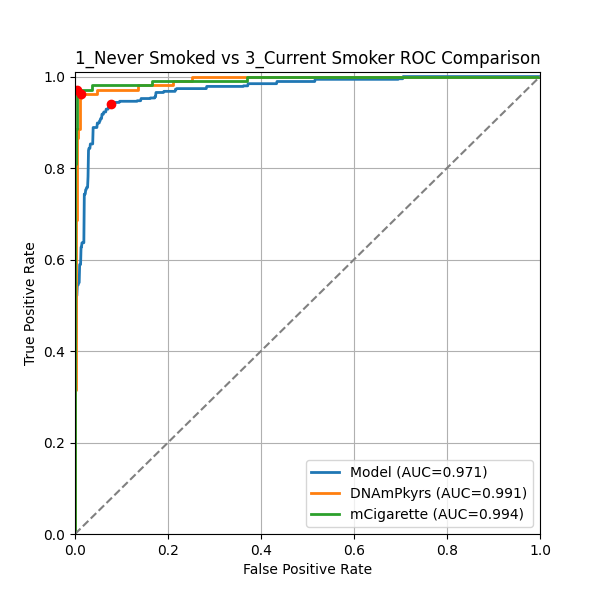
\includegraphics[width=\linewidth]{comparison_1v3_roc.png}
        \caption{comparison 1v3}
    \end{subfigure}
\end{figure}


\begin{figure}
    \centering
    \begin{subfigure}{\textwidth}
        \centering
        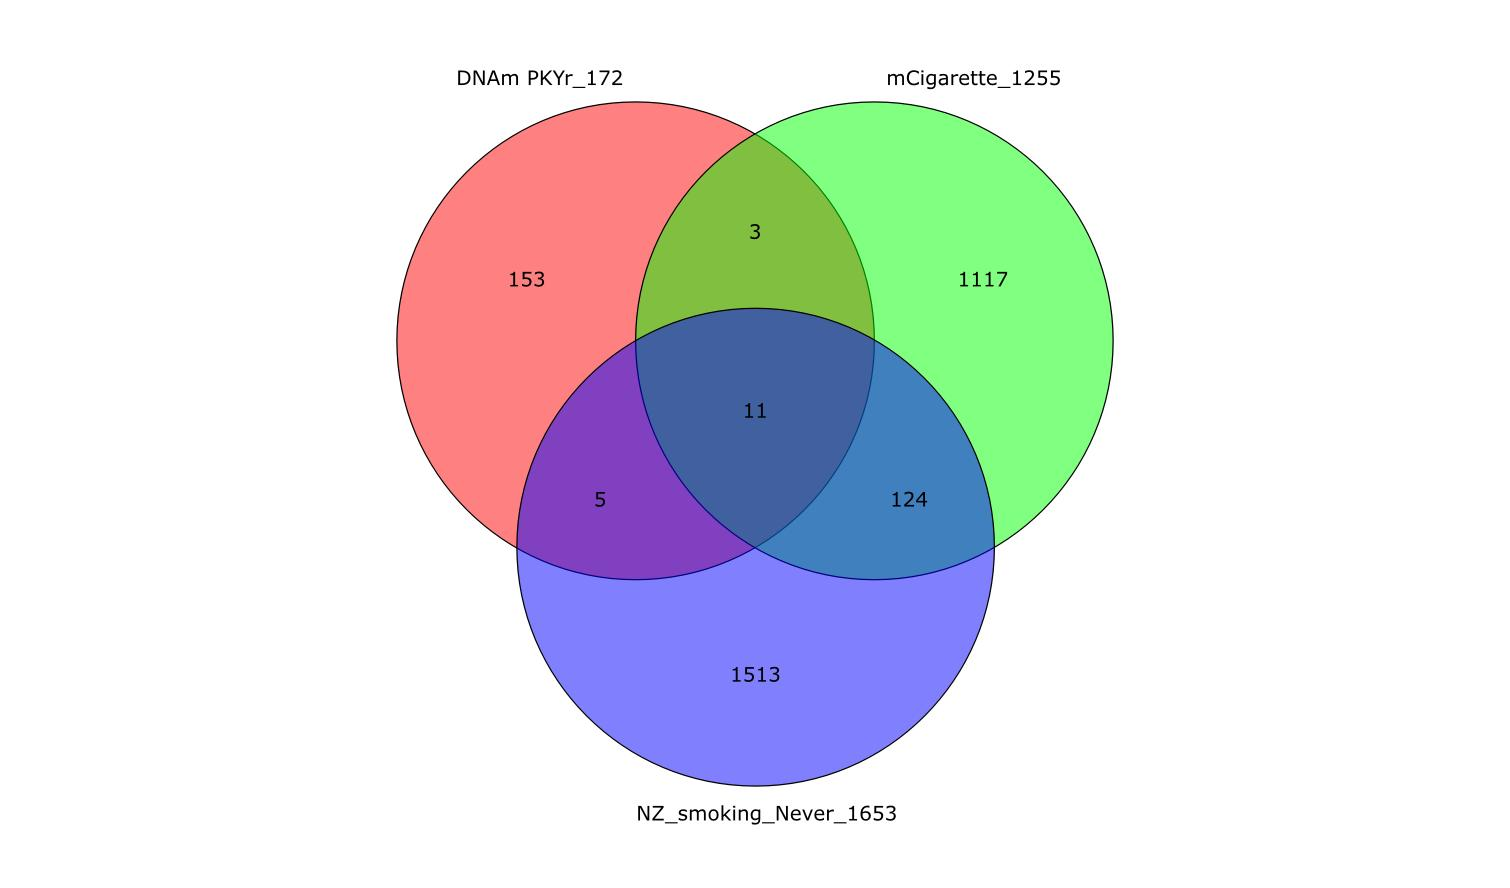
\includegraphics[width=\linewidth]{Venn_NZnever.jpg}
    \end{subfigure}
\end{figure}

\begin{figure}
    \begin{subfigure}{\textwidth}
        \centering
        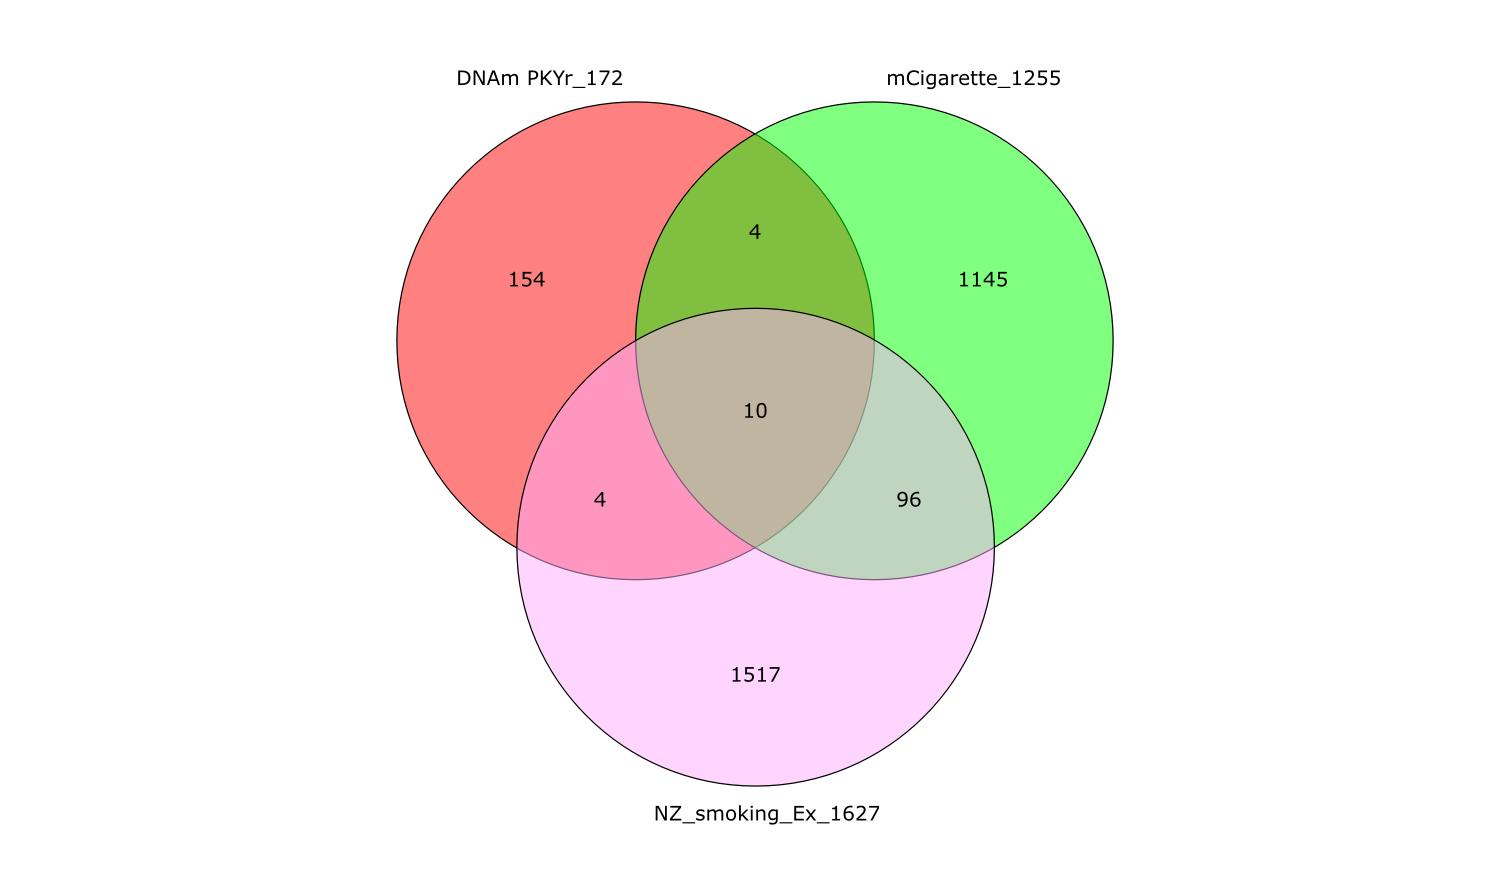
\includegraphics[width=\linewidth]{Venn_NZEx.jpg}
    \end{subfigure}
\end{figure}

\begin{figure}
    \begin{subfigure}{\textwidth}
        \centering
        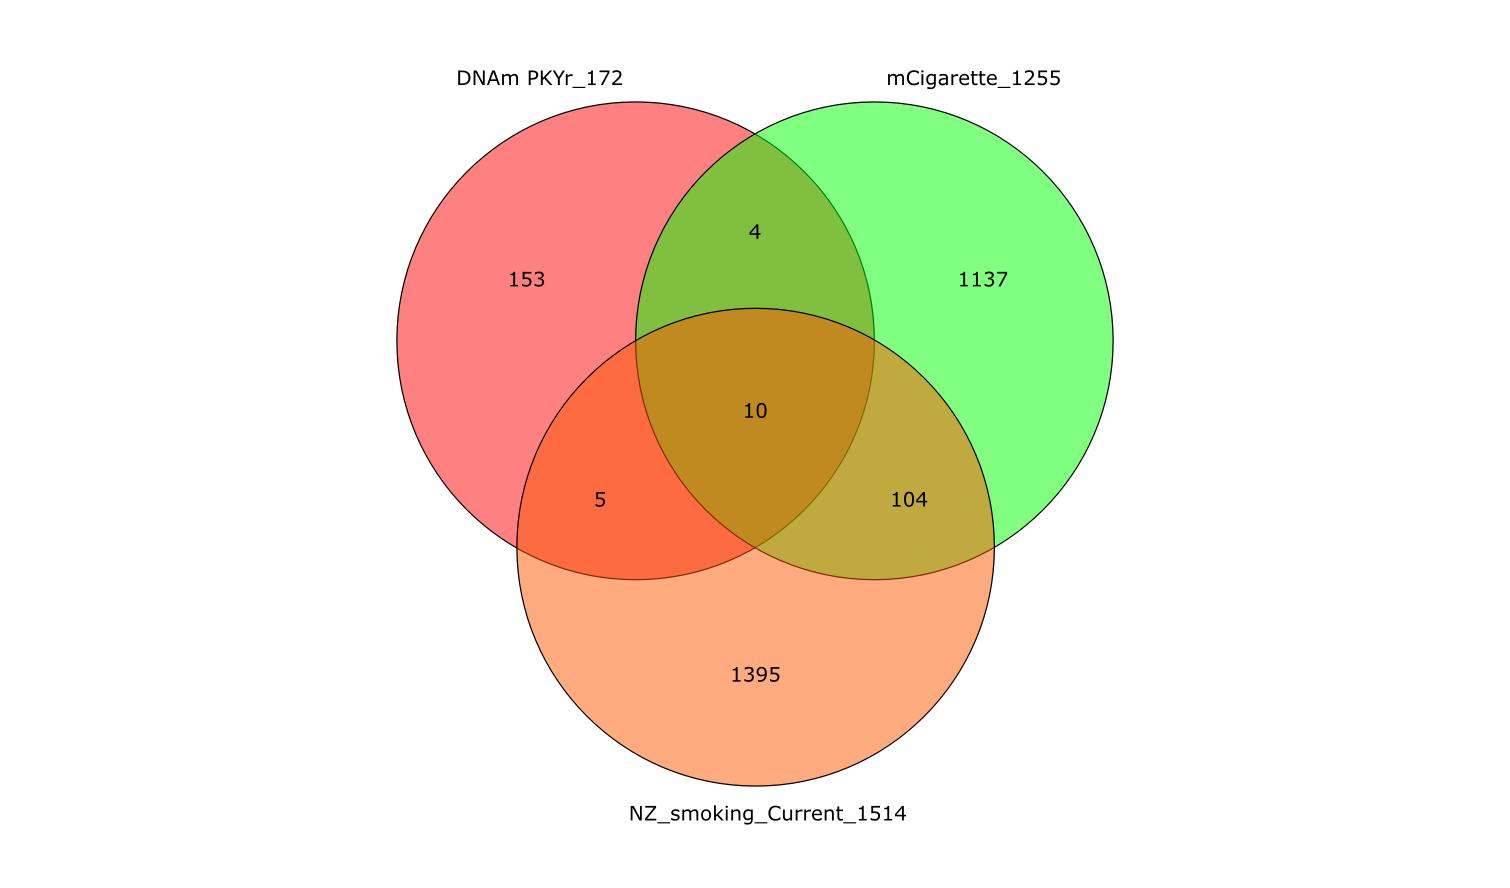
\includegraphics[width=\linewidth]{Venn_NZcurrent.jpg}
    \end{subfigure}
\end{figure}


\begin{figure}
    \centering
    \begin{subfigure}{0.48\textwidth}
        \centering
        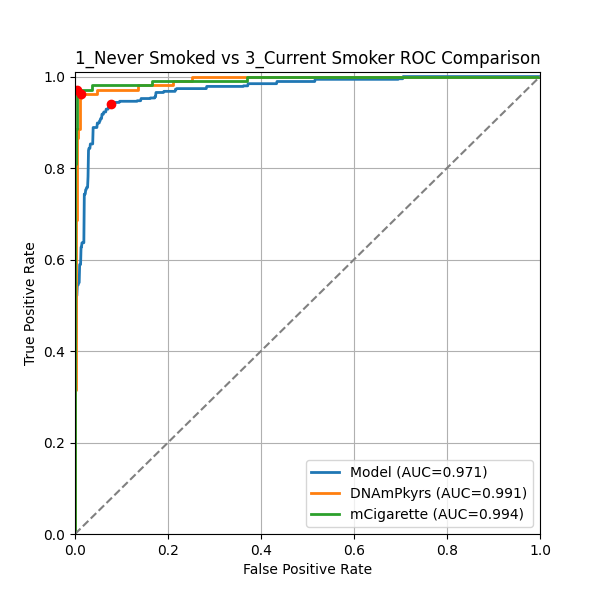
\includegraphics[width=\linewidth]{comparison_1v3_roc.png}
    \end{subfigure}
    \hfill
    \begin{subfigure}{0.48\textwidth}
        \centering
        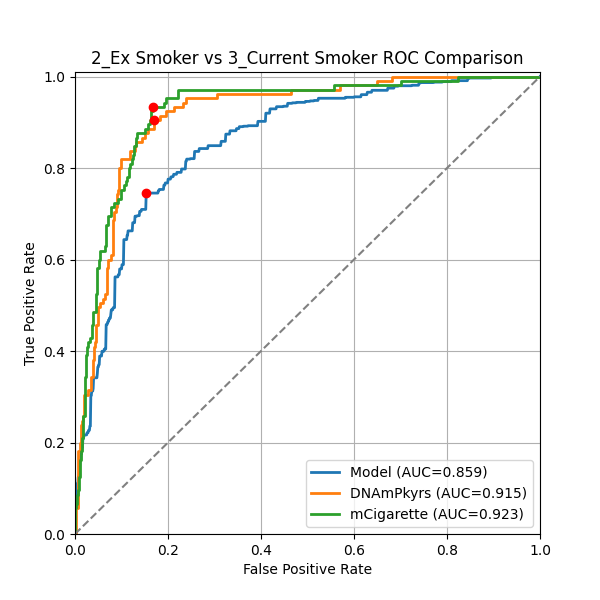
\includegraphics[width=\linewidth]{comparison_2v3_roc.png}
    \end{subfigure}
    \par\vspace{0.5em}
    \begin{subfigure}{0.48\textwidth}
        \centering
        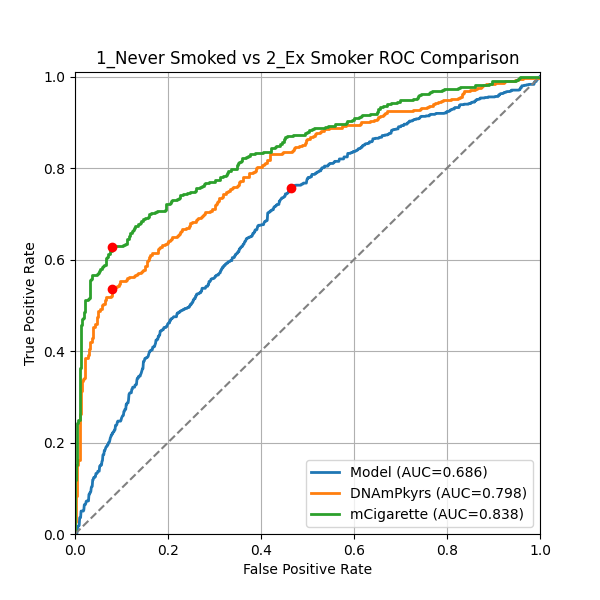
\includegraphics[width=\linewidth]{comparison_1v2_roc.png}
    \end{subfigure}
\end{figure}

\end{document}
